% ================================================================================================================
%  ____            _                                                   
% |  _ \  ___  ___(_) __ _ _ __      _ __  _ __ ___   ___ ___  ___ ___ 
% | | | |/ _ \/ __| |/ _` | '_ \    | '_ \| '__/ _ \ / __/ _ \/ __/ __|
% | |_| |  __/\__ \ | (_| | | | |   | |_) | | | (_) | (_|  __/\__ \__ \
% |____/ \___||___/_|\__, |_| |_|   | .__/|_|  \___/ \___\___||___/___/
%                    |___/          |_|                                
% ================================================================================================================

\section{Поддержка MC-модели с помощью ``Builder'' на протяжении процесса проектирования детектора}\label{sec:DesignProcess}

Использование ``Builder'' для создания и поддержки MC-геометрии на этапе проектирования детектора имеет некоторые особенности. Инженерный проект изменяется и необходимо постоянно поддерживать соответствие MC-модели и САПР-модели. В процессе проектирования можно выделить два вида изменений --- радикальные перемены в структуре и уточнение существующих узлов. В первом случае нередко бывает удобно с нуля перестроить MC-модель, может быть используя некоторые созданные ранее подсборки. Тогда достаточно выделить повторно используемые файлы, описывающие некоторые объёмы, и вставить их в качестве компонентов в верхний документ типа CATProduct разрабатываемой новой геометрии. Если между документами существовала связь типа дочерний-материнский, то она нарушится, т.к. изменится контекст. Для восстановления достаточно выполнить операцию автоматического переопределения связей с помощью операции define contextual links.

В процессе уточнения геометрии иногда возникает необходимость вводить какие-то особенности, которые приводят к невозможности использовать принципы многократного позиционирования объёмов, такие как деление объёмов (секция~\ref{sec:secDivisionReplica}) и массивы (\todo ссылка). Тогда приходится нарушать периодичность структуры, и следовательно краткость описания, и использовать независимые вхождения дочерних объёмов. 

В качестве примера можно привести фокусирующую систему CBM RICH, состоящую из 80~сегментов зеркал шести типов. Для наиболее эффективного описания подобной геометрии следует использовать деление объёма (см. секцию~\ref{sec:secMacroReplica} \todo может быть будет ссылка на секцию про реплику, но не макрос \todo), имеющего форму примитива типа sphere, вдоль кругового направления. Известно, что если использовать деление объёмов, то получается геометрия, более оптимальная с точки зрения времени моделирования прохождения частиц. Исходя из этих соображений, на раннем этапе зеркала фокусирующей системы CBM RICH были созданы следующим образом. Каждое из двух зеркал состояло из трёх сегментов сферы, вытянутых вдоль горизонтальной оси, разделённых на 10~долей вдоль кругового направления, и ещё одной горизонтальной полосы, в которой отдельные сегменты зеркал вставлялись независимо. Дольки, полученные делением каждого из трёх сегментов сферы, соответствуют трём типам сегментов зеркал. 

% \todo Здесь плывёт форматирование. Отследить и исправить!

\begin{minipage}[t]{0.395\textwidth}
\begin{figure}[H]
\centering
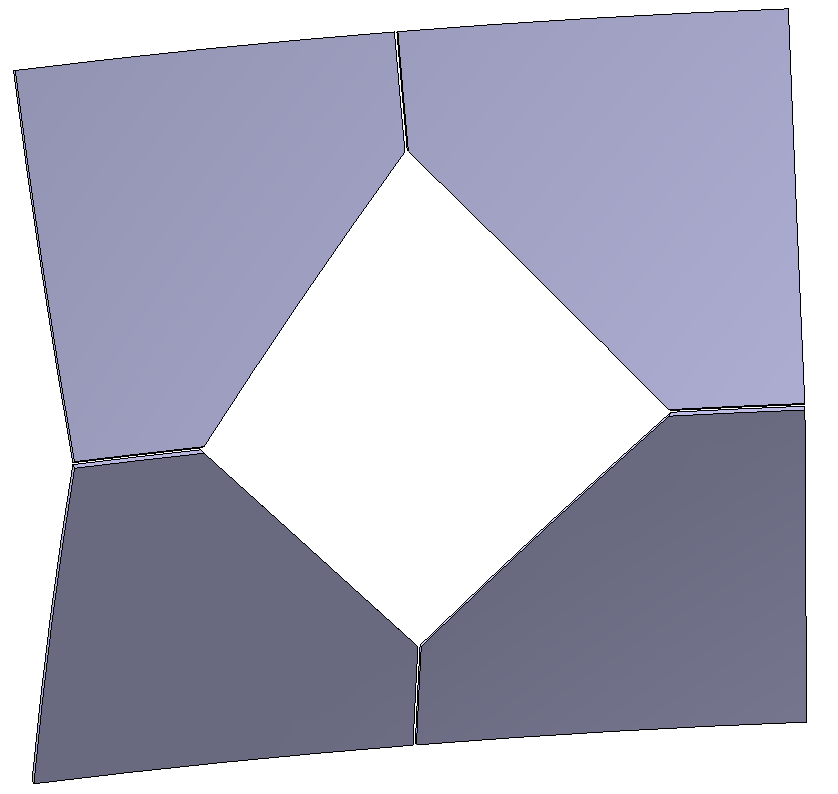
\includegraphics[width=0.7\textwidth]{pictures/Mirror_tiles_special.png}
\caption{Особые сегменты зеркал (type4 и type5), имеющие вырез для ионопровода.}
\label{fig:SpecialMirrorTiles}
\end{figure}
\end{minipage}
\hspace{0.01\textwidth}
\begin{minipage}[t]{0.495\textwidth}
В последней полосе, наиболее близкой к пучку, не было возможности также использовать деление объёма из-за наличия прорези для пучковой трубы. Это привело к тому, что помимо четвёртого типа сегментов зеркал, было введено два дополнительных типа сегментов зеркал, имеющих симметричную форму (см.~\figref{fig:SpecialMirrorTiles}). При таком описании между сегментами зеркал отсутствуют зазоры. Они не были реализованы, т.к. на том этапе эта подробность не имела значения, однако присутствовала возможность легко их добавить введя один дополнительный уровень вложенности.
\end{minipage}

\bigskip

К какой-то момент по мере проработки проекта детектора были зафиксированы параметры зеркал --- радиус, количество и форма сегментов, угол наклона, положение центра, и т.д. Также возникла необходимость выполнять моделирование отклонения индивидуальных сегментов от идеального положения (см. секцию~\ref{sec:secRICHgeoMirror}). Для такого моделирования пользователь должен иметь возможность для каждого сегмента задавать углы отклонения вокруг двух осей в локальной системе координат, индивидуальной для каждого отдельного сегмента. Это требование противоречит идее деления объёмов, где все дольки, полученные в результате деления, имеют одинаковую форму, расположены строго периодически вдоль заданного направления с некоторым шагом и полностью заполняют пространство разделяемого объёма. В случае деления вдоль кругового направления дольки отличаются углом поворота вокруг оси Z и невозможно  задать какое-либо дополнительное вращение каждой отдельной дольке. Таким образом, пришлось отказаться от использования деления объёмов и использовать независимое многократное позиционирование сегментов внутри объёма-контейнера.